\documentclass[11pt]{article}
\usepackage[margin=1in]{geometry}
\usepackage[T1]{fontenc}
\usepackage{lmodern}
\usepackage{amsmath,amssymb,booktabs,array,graphicx}
\usepackage{listings,hyperref}
\setlength{\emergencystretch}{8em}
\makeatletter
\newcommand{\sha}{\begingroup\catcode`\_=12 \sha@read}
\newcommand{\sha@read}[1]{\ttfamily\sha@loop#1\relax\endgroup}
\def\sha@loop#1{%
  \ifx\relax#1\else
    #1\allowbreak
    \expandafter\sha@loop
  \fi}
\makeatother
\hypersetup{colorlinks=true,linkcolor=blue,urlcolor=blue,citecolor=blue,
  pdftitle={Replication of the orthogonal latent-mean contrasts in Jeffries (2024)},
  pdfauthor={}}
\newcommand{\proofcommit}{2dcc1c414311c6a3a4d20cfe25ac390fb97a50cd}
\newcommand{\proofbase}{https://github.com/alectionary/vibe-math/blob/\proofcommit/formalization/latent-contrasts}
\newcommand{\lean}[2]{\href{\proofbase/LatentContrasts/Orthogonality.lean\#L#2}{\texttt{#2}}}
\lstset{basicstyle=\footnotesize\ttfamily,columns=fullflexible,keepspaces=true,
  breaklines=true,showstringspaces=false,frame=single,framerule=.3pt}

\title{Replication of the orthogonal latent-mean contrasts\\
in Jeffries (2024)}
\author{}
\date{27 October 2026}

\begin{document}
\maketitle

\begin{abstract}
When four groups have unequal size, do Jeffries's three latent-mean contrasts stay
orthogonal, and do the Monte Carlo averages sit on the scale of the data-generating
means? Jeffries (2024) defines three codes for four latent means, states that
imbalance makes the set non-orthogonal, and reports multigroup and MIMIC averages
near \(-0.40\), \(-0.20\), and \(0\) when the generating means are
\(1, 0.6, 0.8, 0.4\). We proved the weighted products of the printed codes and the
population values of the printed contrast formulas, and we refit the one-factor
model in lavaan 0.6.17. The codes are orthogonal when the groups are equal. Under
Jeffries's imbalance pattern only the product of the first and third codes is
nonzero. On the generating means the contrasts are \(-2/5\), \(-1/5\), and \(0\).
With the first loading fixed at \(1\), the same formulas give \(-7/25\), \(-7/50\),
and \(0\), and the Monte Carlo averages follow that scale. Fixing the loadings at
\(0.7\), or fixing the factor variance at \(0.50\), brings the averages back near
the printed table. Percent significant is close to Tables~4.1 and~4.2 under either
scale. The analysis script that would decide the identification is not in the
dissertation.
\end{abstract}

\section{What this replication did}
\label{sec:did}

This section answers what we contributed and what we took from Jeffries.
We contributed the orthogonality proofs, the population arithmetic, a lavaan
replay, and Table~\ref{tab:compare}. Jeffries contributed the common-factor
design, the contrast codes, the simulation conditions, and Tables~4.1 through~4.3.
The crops in the later sections are photographs of that dissertation. Every other
number is either a theorem in \texttt{LatentContrasts/Orthogonality.lean} or a
summary of \texttt{simulation/out/}.

The dissertation studies one factor with four indicators. Four groups have latent
means \(\alpha=(1,0.6,0.8,0.4)\) in the true-difference condition and
\(\alpha=(1,1,1,1)\) in the null. Strong invariance is built into the population.
Total sample size is \(240\), \(480\), or \(960\). The group shares are
\(25/25/25/25\), \(35/35/15/15\), and \(45/45/5/5\). Jeffries asks whether
contrasts that are orthogonal at equal sizes stay accurate when the sizes differ,
and compares a multigroup confirmatory factor model with a MIMIC model.

\section{Comparison}
\label{sec:compare}

Table~\ref{tab:compare} puts one published claim on each row. ``Match'' means the
printed value and our value agree as exact numbers or as the same Monte Carlo
target. ``Close'' means our Monte Carlo, at 200 replicates, sits within ordinary
sampling error of the printed average or percent. ``Partial'' means one piece of
the claim holds and another does not. ``No match'' means the two numbers are on
different scales after the checks in Sections~\ref{sec:assumptions}
and~\ref{sec:resolved}.

\begin{table}[ht]
\centering
\small
\begin{tabular}{@{}p{0.26\textwidth}p{0.22\textwidth}p{0.24\textwidth}p{0.16\textwidth}@{}}
\toprule
Claim & Published & Ours & Verdict \\
\midrule
Unweighted products of the Table~2.2 codes &
Equation~(2.4) is zero &
Proved zero &
match \\
Contrasts on \((1, 3/5, 4/5, 2/5)\) &
\(-0.4,\ -0.2,\ 0\) &
\(-2/5,\ -1/5,\ 0\) &
match \\
Third contrast while the means differ &
Used as a null contrast &
Proved equal to \(0\) &
match \\
Imbalance destroys orthogonality &
The set becomes non-orthogonal &
Only code 1 with code 3 fails &
partial \\
Marker scale of those contrasts &
Tables give about \(-0.40,\ -0.20,\ 0\) &
\(-7/25,\ -7/50,\ 0\), and the fits follow it &
no match \\
Loadings fixed at \(0.7\), \(N=20{,}000\) per group &
About \(-0.40,\ -0.20,\ 0\) &
\(-0.398,\ -0.194,\ 0.001\) &
close \\
Factor variance fixed at \(0.50\), same sample &
About \(-0.40,\ -0.20,\ 0\) &
\(-0.400,\ -0.195,\ 0.001\) &
close \\
Table~4.1, \(N=240\), equal groups, percent significant &
\(87.23,\ 35.57,\ 5.29\) &
Marker model, 200 replicates: \(90.5,\ 37.5,\ 4.5\) &
close \\
Table~4.1, \(N=240\), shares \(45/45/5/5\), percent significant &
\(49.23,\ 21.08,\ 7.77\) &
\(52.0,\ 22.5,\ 4.5\) &
partial \\
Table~4.2 MIMIC averages, \(N=240\), equal groups &
\(-0.400,\ -0.200,\ 0.001\) &
Marker MIMIC: \(-0.282,\ -0.136,\ 0.002\) &
no match \\
Same MIMIC cell, loadings fixed at \(0.7\) &
\(-0.400,\ -0.200,\ 0.001\) &
\(-0.406,\ -0.203,\ -0.003\) &
close \\
Numeric codes \(\pm 1\) as covariates, loadings fixed &
The full contrast &
About half: \(-0.195,\ -0.095,\ -0.007\) &
no match \\
Table~4.3, \(N=240\), shares \(45/45/5/5\), percent significant &
\(8.13,\ 8.59,\ 7.73\) &
Marker null model: \(8.5,\ 5.5,\ 9.0\) &
partial \\
\bottomrule
\end{tabular}
\caption{Published claims against this replication. Monte Carlo rows use 200
replicates except the two large-sample rows, which are one sample of \(20{,}000\)
per group.}
\label{tab:compare}
\end{table}

The unweighted-product row is the identity in equation~(2.4), proved at
\lean{}{103}. The population row is equations~(3.3)--(3.5) on the printed means,
proved at \lean{}{123}. The third contrast is zero while the first two means
differ, proved at \lean{}{127}. The imbalance row is partial because
\lean{}{68} shows that the pattern of two equal large groups and two equal small
groups leaves the products of codes 1 with 2, and 2 with 3, at zero, and sets the
remaining product to \(2(b-a)\). At the \(N=240\) sizes that product is \(-96\) in
condition~2 and \(-192\) in condition~3.

The marker row is a no match for the printed averages. Chapter~III fixes the
first loading at \(1\) and frees the factor variances. Under the data-generating
loading \(0.7\), the contrasts on that scale are \(-7/25\), \(-7/50\), and \(0\),
proved at \lean{}{131}. Two hundred marker replicates at \(N=240\) in the equal
true-difference cell averaged \(-0.286\), \(-0.134\), and \(0.007\). The printed
Table~4.1 cell averages \(-0.4046\), \(-0.2027\), and \(-0.0010\). The page crop
and the text layer agree on both the marker sentence and the table, so the gap is
not an extraction error. Turning the marker constraint off, by fixing every
loading at \(0.7\) or by fixing the factor variance at \(0.50\), moves our
averages onto the printed scale. Those two rows are therefore close, and the
marker row stays a no match. The same split appears in the MIMIC block: a
marker MIMIC misses the printed averages, and a MIMIC with loadings fixed at
\(0.7\) is close.

Percent significant can agree while the averages do not. Multiplying a contrast
and its standard error by \(0.7\) leaves the \(z\) statistic unchanged. The equal
true-difference percents in Table~4.1 are close to the marker replay. In the
\(45/45/5/5\) cell the first two percents are close and the third, \(4.5\) against
\(7.77\), is not, at 200 replicates, so that row is partial. The null percents in
Table~4.3 are partial for the same reason: \(8.5\) is close to \(8.13\), while
\(5.5\) and \(9.0\) sit off \(8.59\) and \(7.73\). A binomial standard error at
200 replicates and a rate near \(0.08\) is about two percentage points.

The numeric-code row is a no match to the printed averages. With the codes stored
as numbers, the slope is about half the defined contrast, because the code
changes by \(2\). With the codes stored as factors whose levels are \(-1\) and
\(1\), lavaan's treatment contrast estimates the full difference. The appendix
stores the codes as factors. The half-size slopes are what the numeric coding
does, not what Table~4.2 prints.

\section{Assumptions}
\label{sec:assumptions}

Each subsection is a choice the dissertation does not pin down and that this
replay supplied.

\subsection{Random-number stream}

Jeffries sets \texttt{set.seed(1313)} and passes seed \(13131\) to
\texttt{exportData}. We drew normal factor scores and normal residuals in R with
the L'Ecuyer generator and \texttt{set.seed(13131)}. The replicates are not
Jeffries's replicates. Agreement is about the Monte Carlo mean, not about a
shared sample.

\subsection{R version and the optimizer}

The dissertation names R~4.2.2, simsem~0.5.16, and lavaan~0.6.17, with estimator
MLR and up to \(10{,}000\) iterations. We used R~4.3.3 and lavaan~0.6.17. We did
not call simsem. The optimizer is lavaan's default \texttt{nlminb}, with
\texttt{iter.max} set to \(1{,}000\). A fit counts as a success when it
converges and the three contrast standard errors are finite.

\subsection{Replicate count}

Jeffries keeps \(10{,}000\) converged replicates in each cell, after drawing
\(15{,}000\). We used \(200\) replicates for every \(N=240\) cell in the main
grid and in the identification check, and \(100\) replicates at \(N=960\). The
large-sample rows are one dataset with \(20{,}000\) observations in each group.
Percents from \(200\) replicates are coarser than percents from \(10{,}000\).

\subsection{Intercept of the first indicator}

Appendix~A writes \texttt{i1 \textasciitilde\ 1*} and
\texttt{i2 \textasciitilde\ 1*1}, and the same \texttt{1*1} form for the third
and fourth indicators. lavaan~0.6.17 rejects \texttt{i1 \textasciitilde\ 1*} as
a formula. We fixed every intercept at \(1\), which is the value printed for the
other three indicators and the value named in the population description.

\subsection{Sign of the third code}

Table~2.2 codes the third contrast as \(+1,-1,-1,+1\). Appendix~A codes it as
\(-1,+1,+1,-1\). We used the table. Section~\ref{sec:sign} records why the
population value does not depend on that choice.

\subsection{Data-generating variances}

The population paragraph says the loading \(0.70\) accounts for \(49\%\) of the
indicator variance. The appendix sets the loading to \(0.7\), the factor
variance to \(0.5\), and the residual variance to \(0.51\). We generated data
from those three appendix numbers. The squared loading \(0.49\) is then the
explained variance only if the factor variance is \(1\) and the residual is
\(1-0.49\). That is not the appendix.

\section{Ambiguities that were resolved}
\label{sec:resolved}

\subsection{The ink matches the text layer}

The question was whether a sign or a printed average in the text extract
disagreed with the page. It does not, on the pages that carry the claims in
Table~\ref{tab:compare}.

The artifact is the set of PNG crops in
\texttt{formalization/latent-contrasts/paper/figures/}. The script is
\texttt{paper/figures/crop\_pages.py}. It runs \texttt{pdftoppm -png -r 600}.
Pages whose PDF rotation flag is \(90\) degrees are turned clockwise into
reading order before the crop. The command is
\texttt{python3 formalization/latent-contrasts/paper/figures/crop\_pages.py},
and the output is those PNG files. The commit that contains the script is
\proofcommit.

\begin{figure}[ht]
\centering
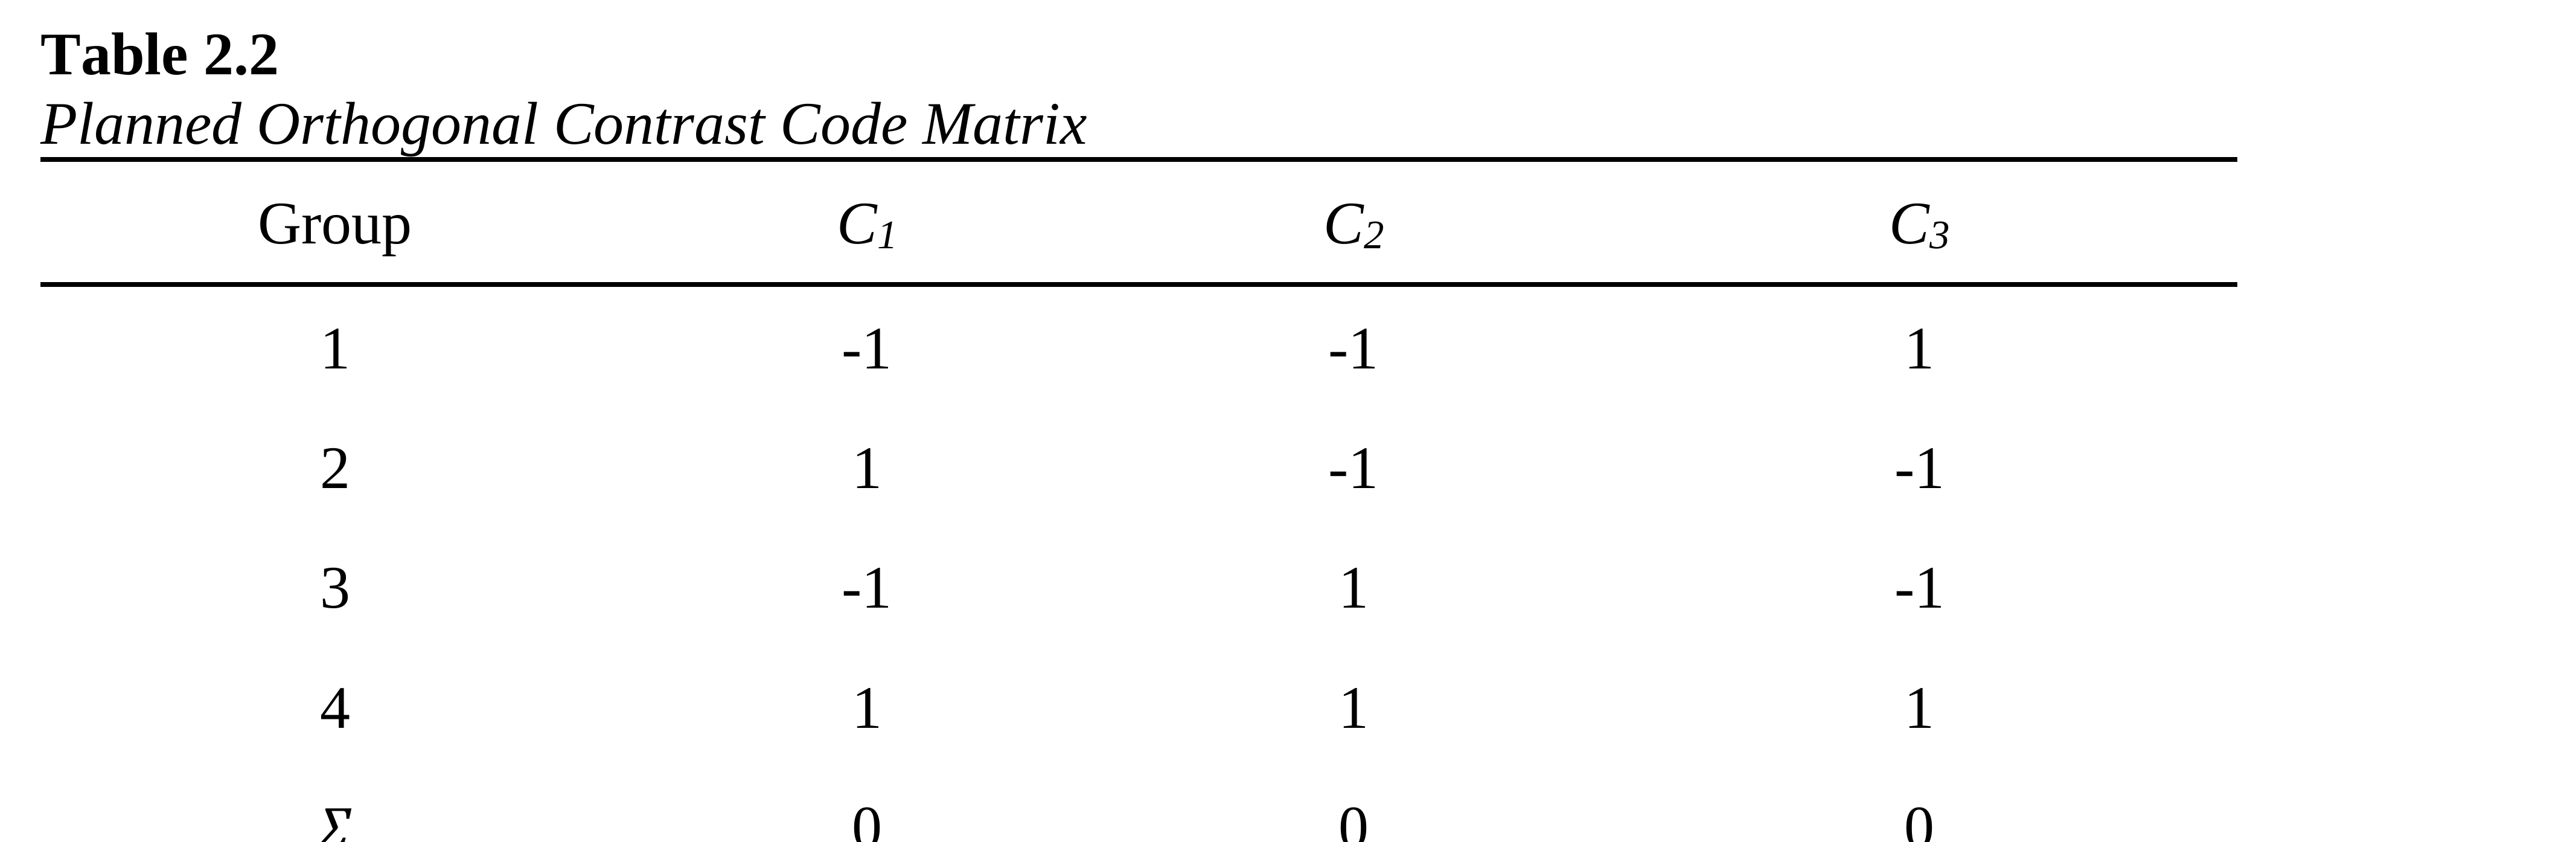
\includegraphics[width=\textwidth]{figures/table22.png}
\caption{Table~2.2. Codes \(C_1=(-1,1,-1,1)\), \(C_2=(-1,-1,1,1)\),
\(C_3=(1,-1,-1,1)\).}
\end{figure}

\begin{figure}[ht]
\centering
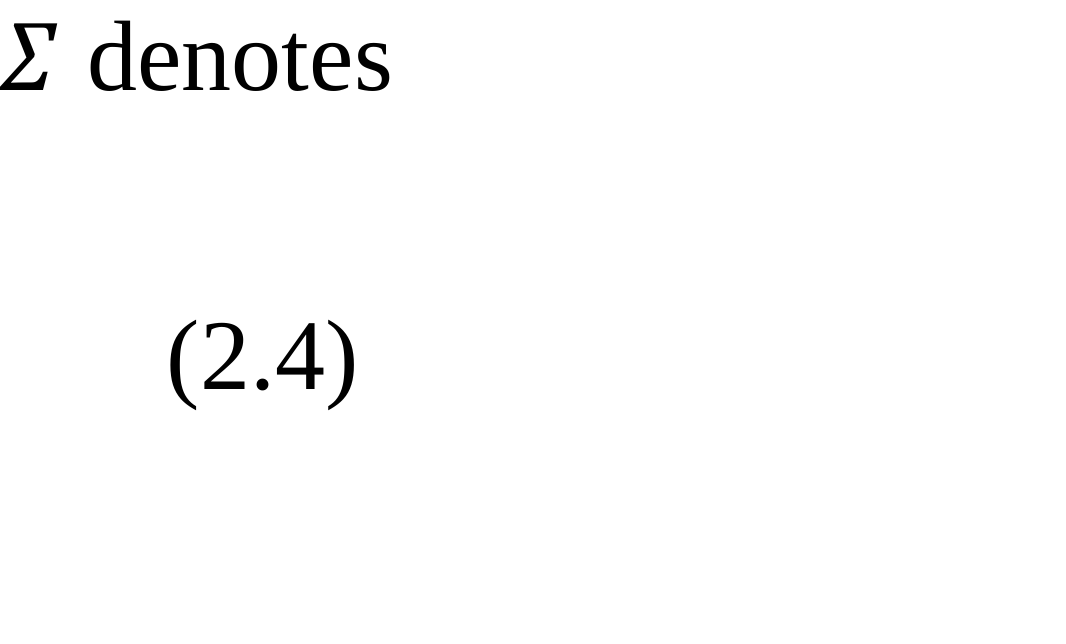
\includegraphics[width=0.9\textwidth]{figures/eq24.png}
\caption{Equation~(2.4). The three unweighted cross-products are zero.}
\end{figure}

\begin{figure}[ht]
\centering
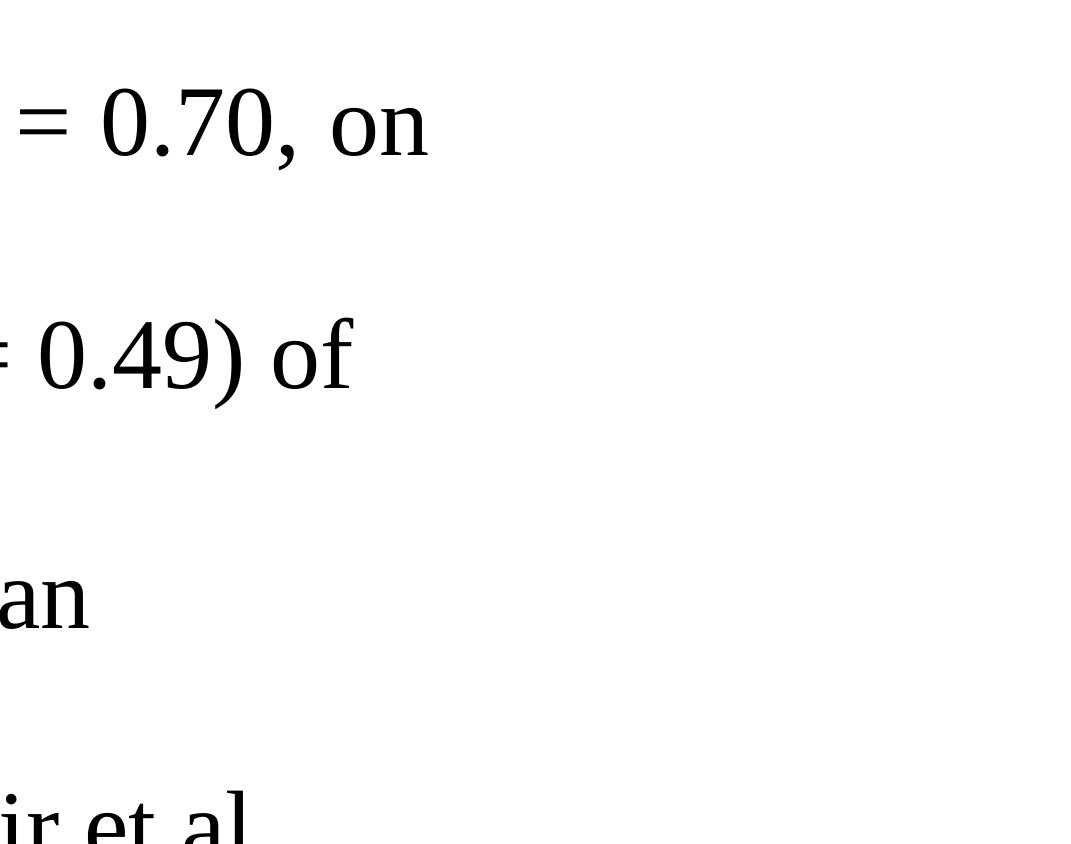
\includegraphics[width=0.85\textwidth]{figures/population.png}
\caption{Population loadings \(0.70\), means \((1, 0.6, 0.8, 0.4)\), and factor
variance \(0.50\).}
\end{figure}

\begin{figure}[ht]
\centering
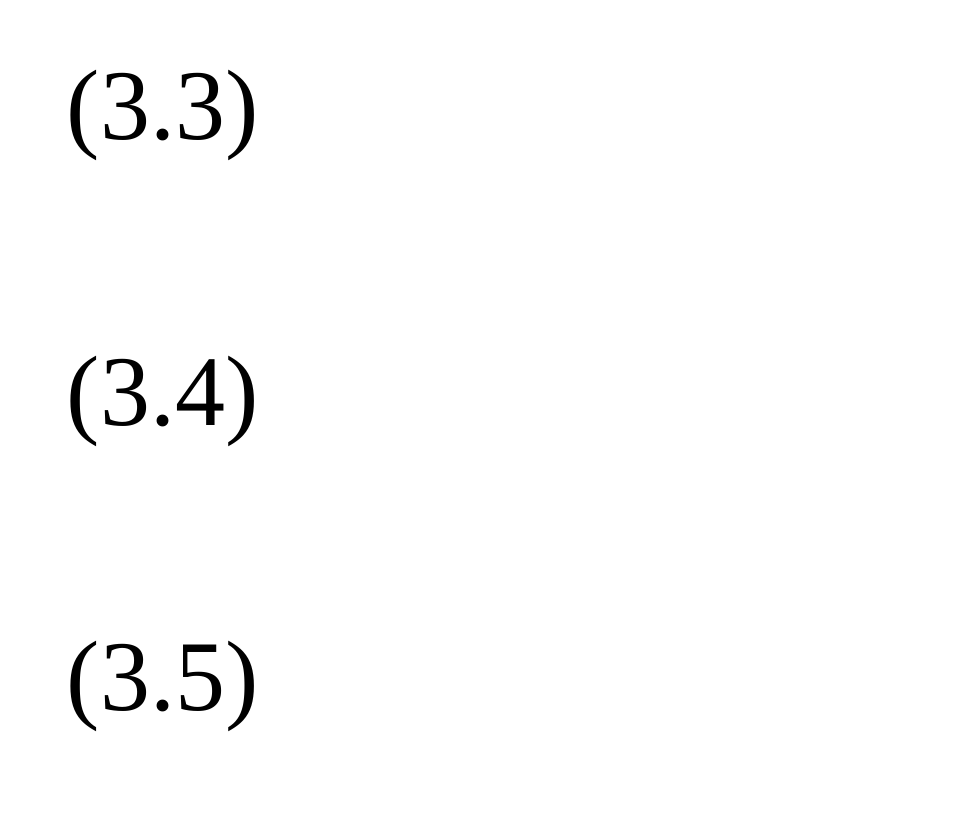
\includegraphics[width=0.9\textwidth]{figures/eq33.png}
\caption{Equations~(3.3)--(3.5). Each contrast is the mean of the groups coded
\(+1\), minus the mean of the groups coded \(-1\).}
\end{figure}

\begin{figure}[ht]
\centering
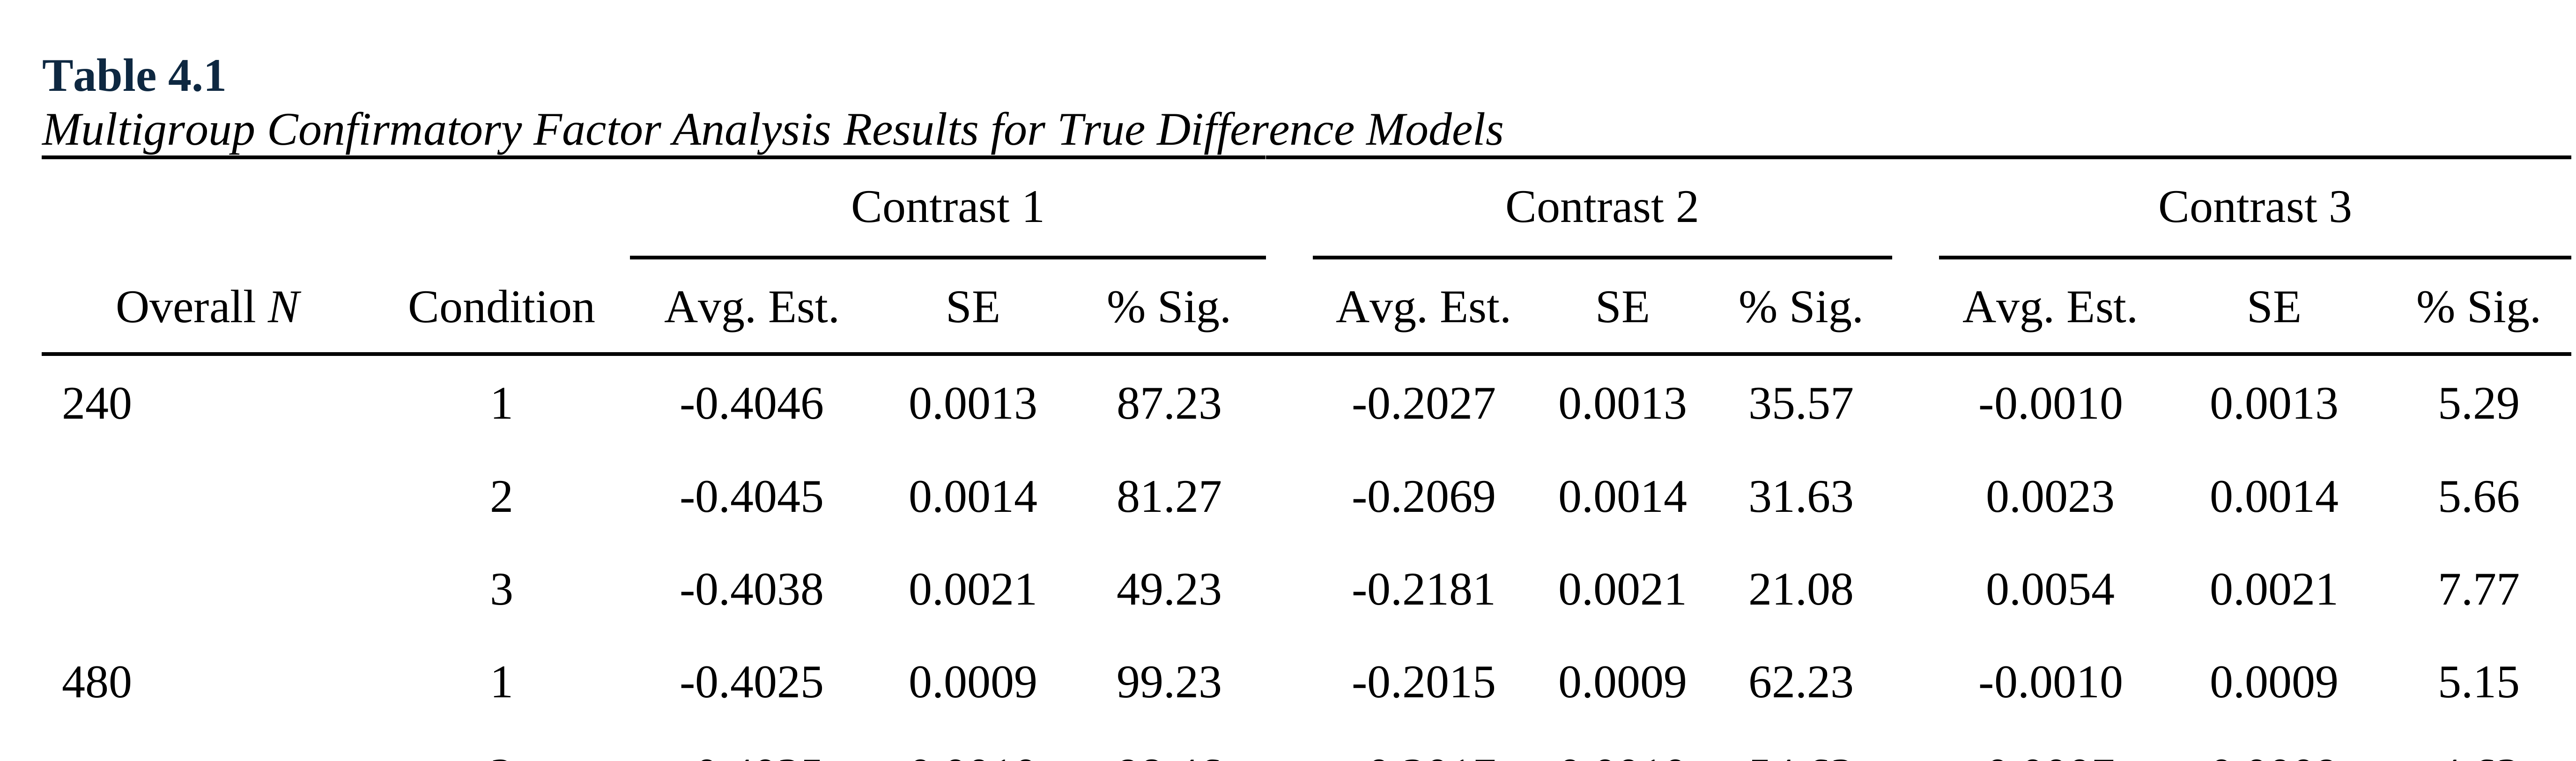
\includegraphics[width=\textwidth]{figures/table41.png}
\caption{Table~4.1, multigroup model, true difference. At \(N=240\) and equal
groups the averages are \(-0.4046\), \(-0.2027\), and \(-0.0010\).}
\end{figure}

\begin{figure}[ht]
\centering
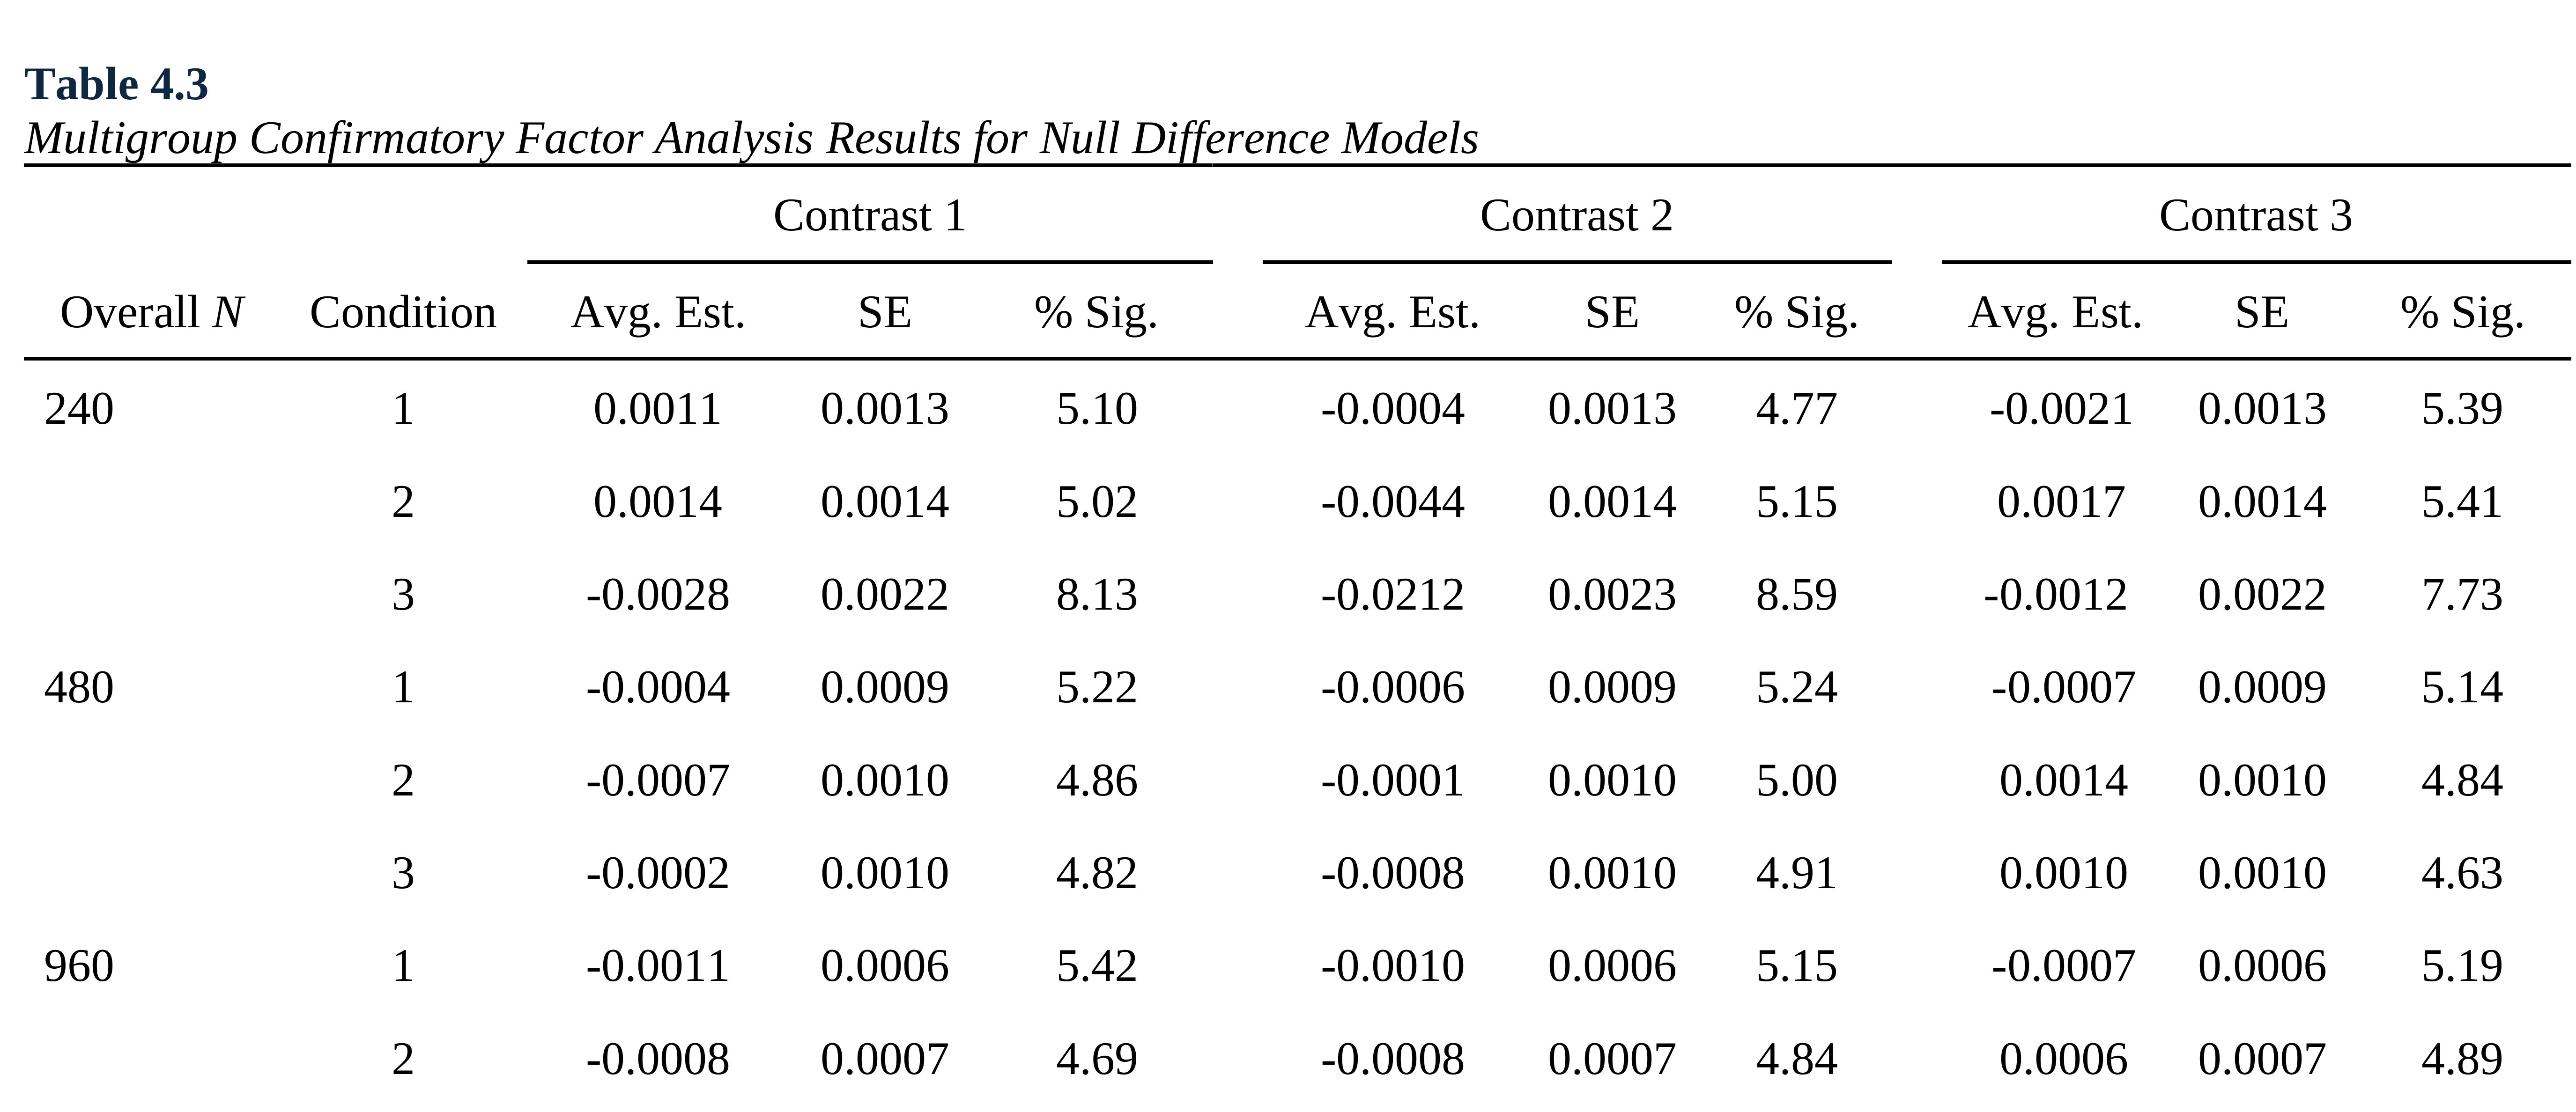
\includegraphics[width=\textwidth]{figures/table43.png}
\caption{Table~4.3, multigroup model, null difference. At \(N=240\) and shares
\(45/45/5/5\) the percents significant are \(8.13\), \(8.59\), and \(7.73\).}
\end{figure}

The standard-error column in these tables is about \(0.001\) to \(0.002\). That
is the standard error of a mean of \(10{,}000\) replicates, not the average
within-replicate standard error. Our column \texttt{sd\_est} is the standard
deviation across replicates, about \(0.08\) to \(0.14\) at \(N=240\), and is not
compared with that printed column.

\subsection{The third code in the appendix}
\label{sec:sign}

The question was whether Appendix~A uses the Table~2.2 sign for the third code.
It uses the opposite sign.

\begin{figure}[ht]
\centering
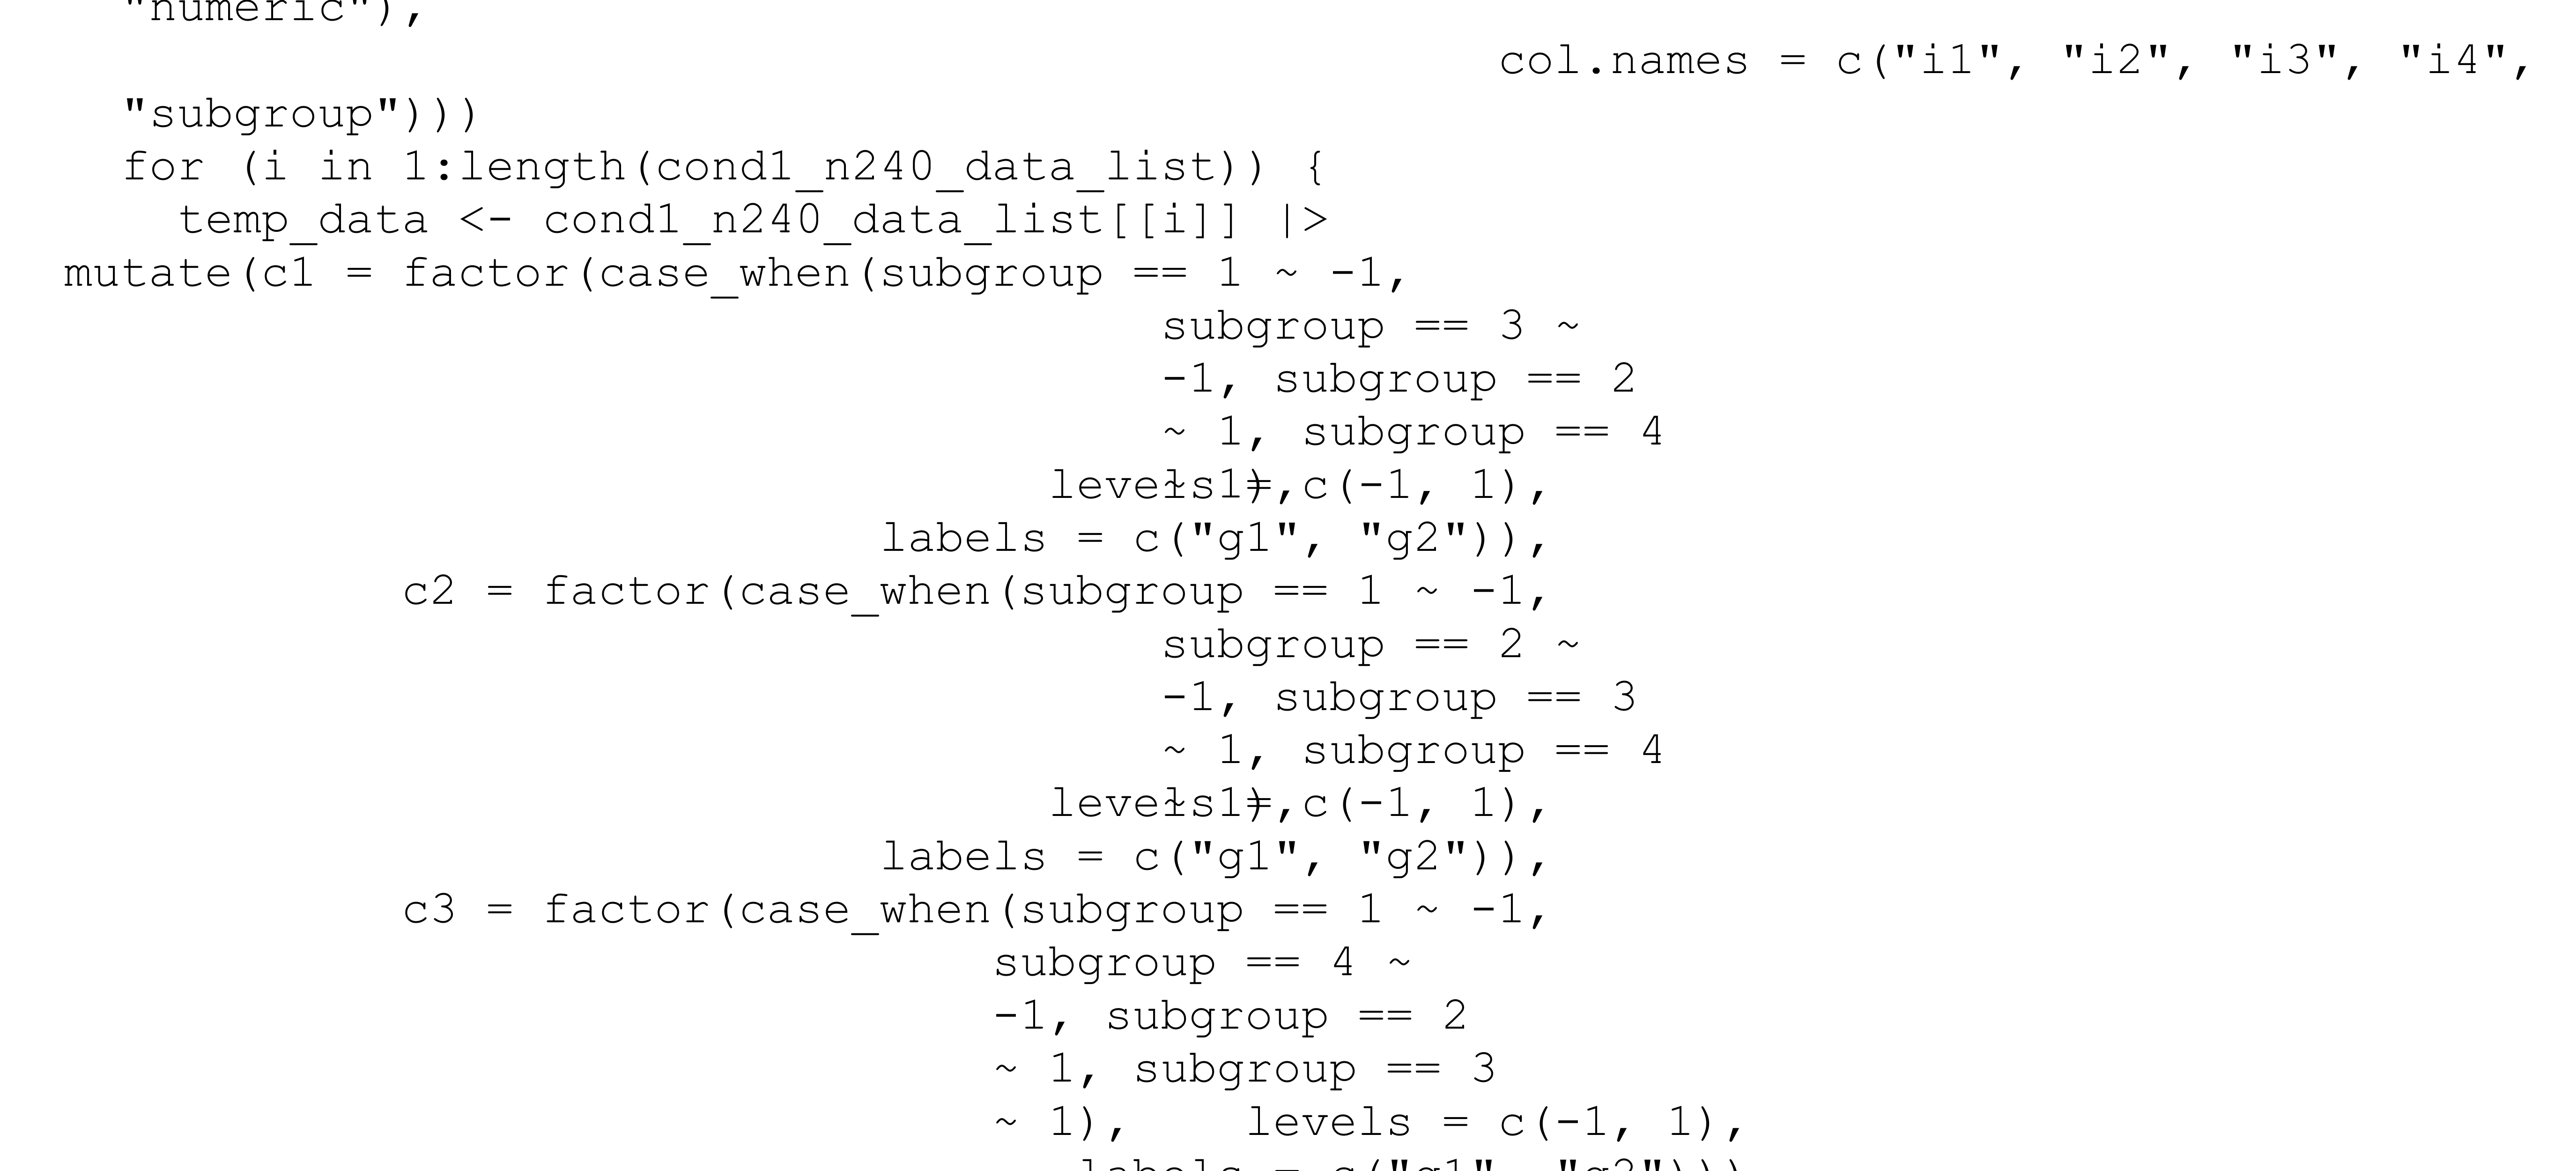
\includegraphics[width=\textwidth]{figures/appendix_c3.png}
\caption{Appendix~A. Groups 1 and 4 are coded \(-1\) on \texttt{c3}, and groups
2 and 3 are coded \(+1\). Codes \texttt{c1} and \texttt{c2} match Table~2.2.}
\end{figure}

The artifact is \texttt{figures/appendix\_c3.png}, produced by the same script,
output, and commit as the previous subsection. On the printed means the third
contrast is zero, so changing the sign leaves the population value at zero and
does not move a percent-significant column for a two-sided test of that
contrast. The replay uses the table's sign.

\subsection{Factor coding against numeric coding}

The question was whether a covariate coded \(\pm 1\) estimates the contrast in
equations~(3.3)--(3.5) or half of it. As a factor with levels \(-1\) and \(1\),
lavaan's treatment contrast estimates the full difference. As a number, the
slope is half of that difference, because the code changes by \(2\).

The check is \texttt{simulation/identification\_check.R}, model
\texttt{mimic\_numeric}, output
\texttt{simulation/out/identification\_check.csv}. The command is
\texttt{Rscript identification\_check.R 200 out} from
\texttt{formalization/latent-contrasts/simulation}. The commit is
\proofcommit. At \(N=240\), equal groups, loadings fixed at \(0.7\), and \(200\)
replicates, the numeric slopes averaged \(-0.195\), \(-0.095\), and \(-0.007\).
The factor version of the same model averaged \(-0.406\), \(-0.203\), and
\(-0.003\). Theorem \lean{}{159} shows that the full contrasts \(-2/5\) and
\(-1/5\), entered as treatment coefficients on the \(0/1\) recoding of
Table~2.2, recover the four printed means.

\subsection{Which scale the averages use}

The question was which identification puts the fitted contrasts on the scale of
Table~4.1. Three identifications were fit on the same draws.

The script, output, command, and commit are the same as the previous
subsection. The marker multigroup model fixes the first loading at \(1\),
equates loadings and intercepts, and frees four means. Two hundred replicates
averaged \(-0.286\), \(-0.134\), and \(0.007\). One sample with \(20{,}000\) per
group gave \(-0.277\), \(-0.135\), and \(0.000\). The marker population is
\(-0.28\), \(-0.14\), and \(0\).

The fixed-measurement model fixes every loading at \(0.7\) and every intercept
at \(1\). The same \(20{,}000\)-per-group sample gave \(-0.398\), \(-0.194\),
and \(0.001\). Two hundred replicates at \(N=240\) averaged \(-0.390\),
\(-0.206\), and \(-0.010\).

The variance-fixed model frees the loadings, fixes the factor variance at
\(0.50\), and equates loadings and intercepts. The large sample gave
\(-0.400\), \(-0.195\), and \(0.001\).

Chapter~III describes the marker constraints. Tables~4.1 and~4.2 print the
generating scale. Both statements are on the page. The replay shows which
constraint produces which scale. It does not decide which constraint Jeffries
fit. The analysis syntax is not in Appendix~A. That request is recorded as a
help issue, linked in Section~\ref{sec:availability}.

\subsection{The first intercept token}

The question was whether the text extract had dropped a digit from
\texttt{i1 \textasciitilde\ 1*}. The ink is \texttt{1*}. The next three
intercepts are \texttt{1*1}.

\begin{figure}[ht]
\centering
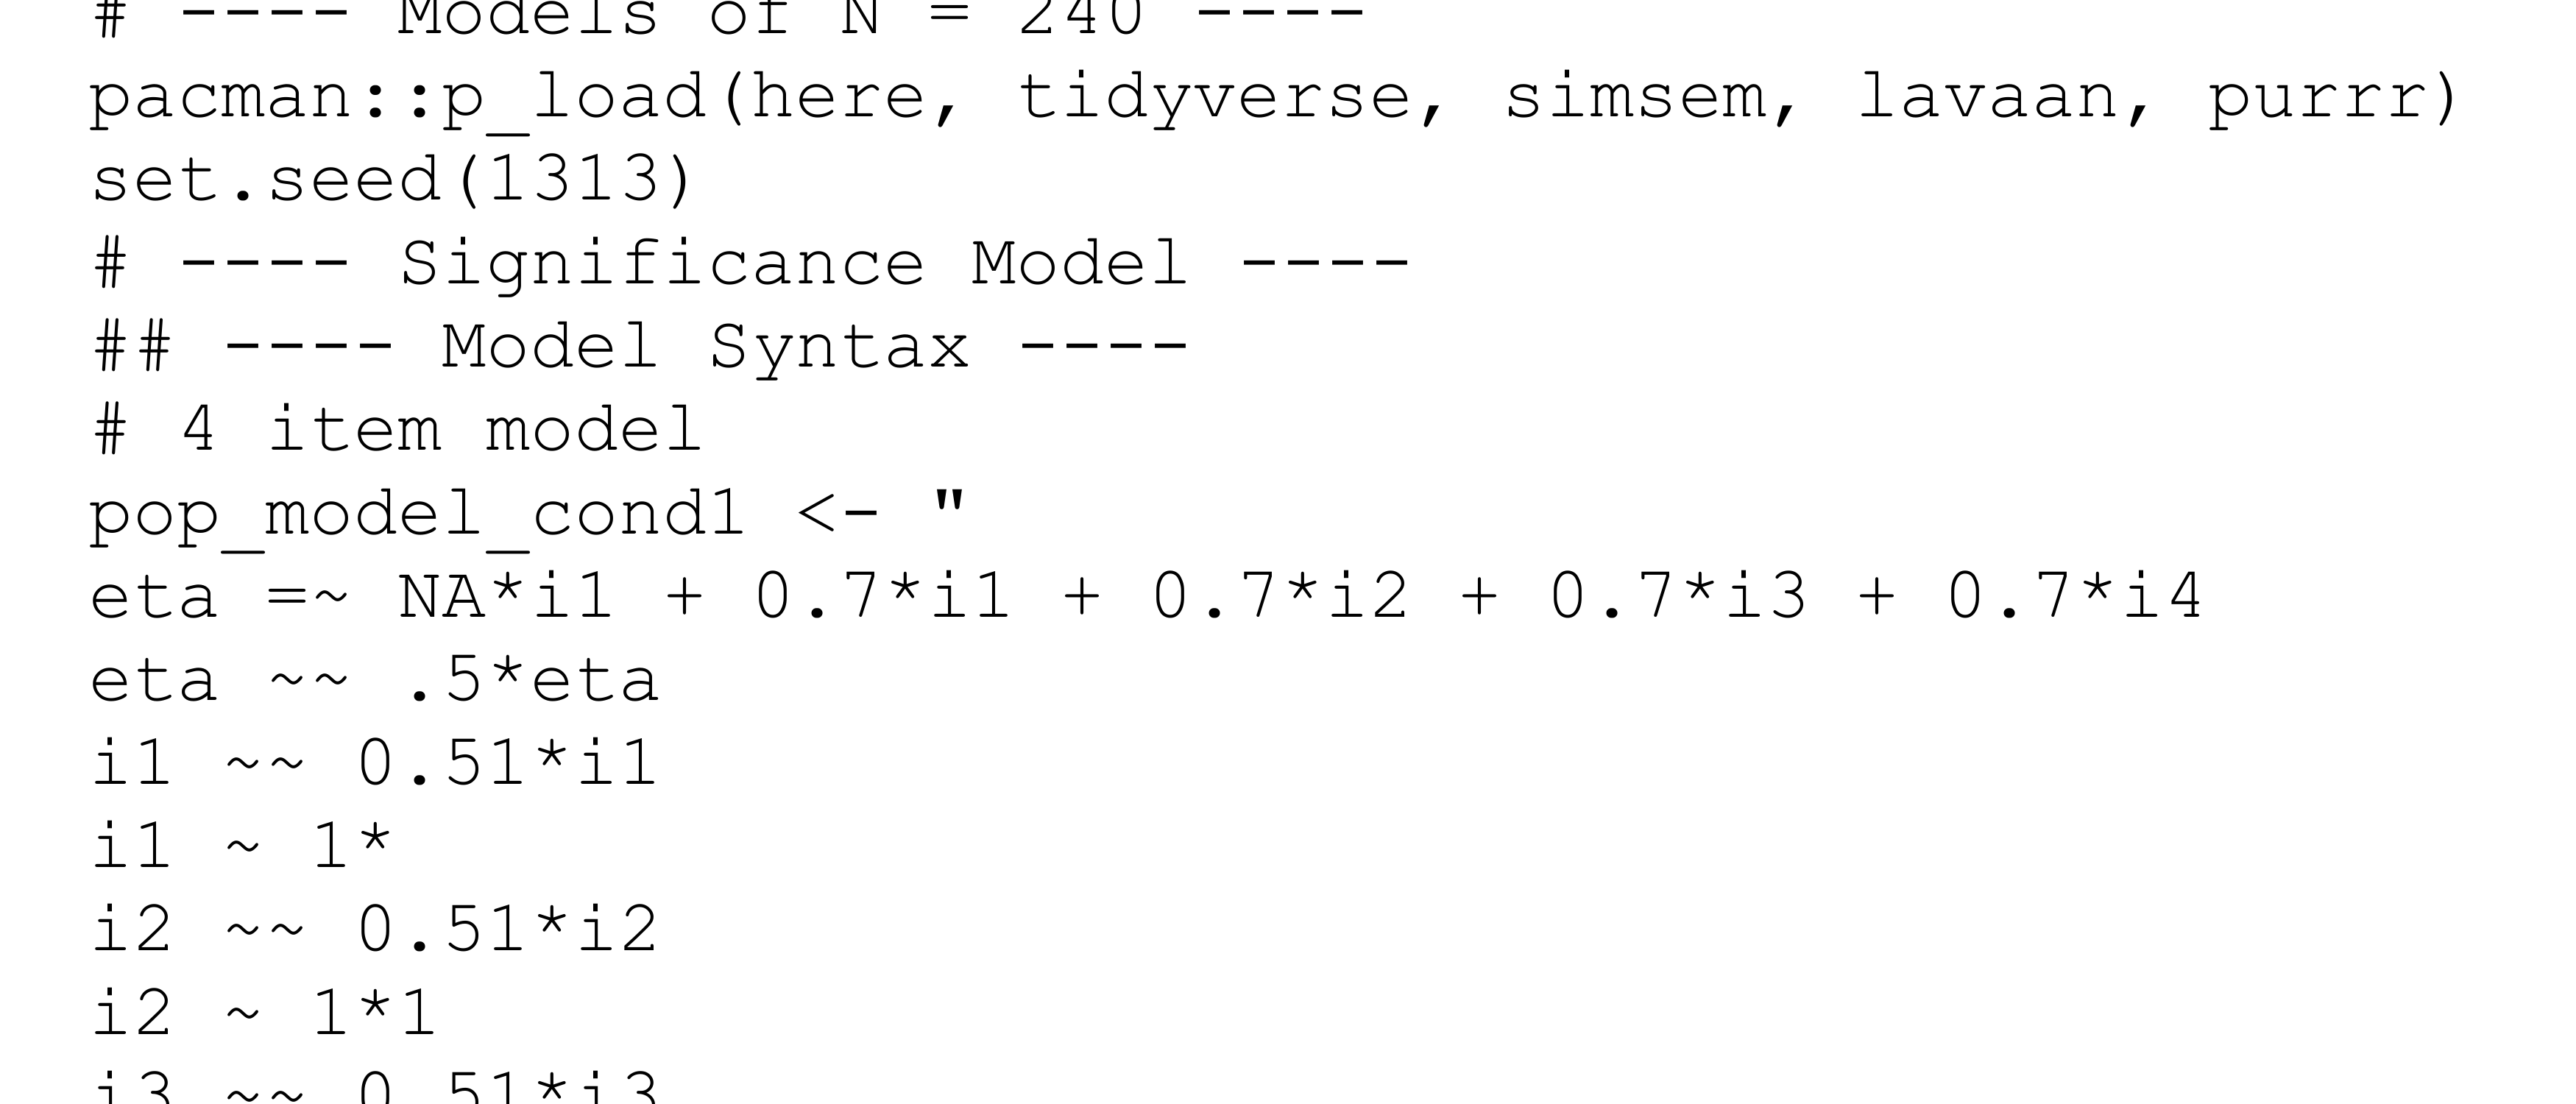
\includegraphics[width=\textwidth]{figures/appendix_intercept.png}
\caption{Appendix~A population model. The first intercept is written
\texttt{1*}. The loading line contains both \texttt{NA*i1} and
\texttt{0.7*i1}.}
\end{figure}

The artifact is \texttt{figures/appendix\_intercept.png}, from the same script
and commit. We did not find a second digit on that line. lavaan~0.6.17 does
not parse \texttt{i1 \textasciitilde\ 1*}. simsem~0.5.16 was not run, so this
does not say what simsem does with the token. Data generation in the replay
used intercept \(1\) for every indicator.

\section{What remains unresolved}
\label{sec:unresolved}

The analysis syntax is unresolved. The marker sentence and the printed averages
cannot be true of the same fitted contrast, on the population this appendix
generates. Three candidates still fit the tables: loadings fixed at the
data-generating value, factor variance fixed at \(0.50\), or a report of the
contrasts after they have been divided by the estimated loading. The third was
not fit here. Percent significant does not separate them. The missing script is
issue \url{https://github.com/alectionary/vibe-math/issues/33}.

Convergence is unresolved. Table~4.5, as read from the text layer, reports
\(8{,}929\) of \(10{,}000\) converged multigroup significance models at
\(N=240\) and shares \(45/45/5/5\). All \(200\) of our marker fits in that cell
converged, with \texttt{iter.max} of \(1{,}000\). We did not draw \(15{,}000\)
simsem datasets, and we did not use the iteration cap of \(10{,}000\). The rate
\(89.29\%\) is therefore not a number this replay tested.

The \(200\)-replicate gaps in the third contrast's percent, in the unbalanced
null cell and in the unbalanced true-difference cell, may shrink at
\(10{,}000\) replicates. They may also be a feature of the marker standard
errors. The replay cannot tell those apart at this size.

Jeffries and Bovaird (2026) is the journal version of this design. The PDF was
not obtained. Routes are in Section~\ref{sec:availability}. The dissertation
comparison does not use that article.

The token \texttt{NA*i1 + 0.7*i1} was not passed through simsem. Our generator
used the loading \(0.7\) once. If simsem treats the duplicated loading as
something other than \(0.7\), the population would change. Nothing in the
printed loading sentence suggests that.

\section{Code and source availability}
\label{sec:availability}

This section copies the ledger dated 2026-10-27. A row is a place we opened,
not a recollection.

\begin{center}
\small
\begin{tabular}{@{}p{0.42\textwidth}p{0.18\textwidth}p{0.32\textwidth}@{}}
\toprule
Place & Date & Result \\
\midrule
Appendix~A of the dissertation PDF & 2026-10-27 &
Generation syntax only. sha256 of the PDF is
\texttt{a21df98c\ldots fd469b3} \\
GitHub repository search for the dissertation title & 2026-10-27 &
0 repositories \\
GitHub code search for Jeffries and orthogonal latent & 2026-10-27 &
HTTP 429, so not an absence \\
OSF nodes with the dissertation title & 2026-10-27 &
0 nodes \\
OSF \texttt{/v2/search/} & 2026-10-27 & HTTP 404 \\
Sage page for DOI \texttt{10.1177/01466216261452255} & 2026-10-27 &
HTTP 403 \\
Unpaywall for that DOI & 2026-10-27 &
PubMed abstract only, no PDF \\
Europe PMC for that DOI & 2026-10-27 &
Not open access, no PDF \\
Wayback for that DOI & 2026-10-27 & No snapshot \\
PMC13179297 & 2026-10-27 &
HTTP 403, embargo named through 2027-05-15 \\
lavaan 0.6.17, as named in the dissertation & 2026-10-27 &
Installed and used \\
simsem 0.5.16 and dynamic 1.1.0 & 2026-10-27 &
Not installed. The authors' scripts are not those packages \\
\bottomrule
\end{tabular}
\end{center}

The dissertation file itself was retrieved from the Wayback \texttt{id\_}
object dated 2025-05-11, snapshot \texttt{20250511025154}, of the
DigitalCommons \texttt{viewcontent} URL for \texttt{dissunl} article 1215.
The archive landing page is
\url{https://digitalcommons.unl.edu/dissunl/216/}.
Direct \texttt{viewcontent} returned HTTP 403. The help request for the
analysis script is
\url{https://github.com/alectionary/vibe-math/issues/33}.
The fetch request for the 2026 article is
\url{https://github.com/alectionary/vibe-math/issues/34}.

\section{Next steps}

The next check is the analysis function that produced Tables~4.1 and~4.2.
With that syntax, refit one large sample and see whether the contrasts land
near \(-0.40\) or near \(-0.28\). The same script would show the iteration
settings behind the \(8{,}929/10{,}000\) convergence count. The 2026 article
would show whether the published paper uses the same tables. Neither file is
required to trust the orthogonality proof, which uses only the printed codes
and means.

\section{What we proved}

The codes, in group order \((1,2,3,4)\), are
\[
c_1=(-1,1,-1,1),\qquad
c_2=(-1,-1,1,1),\qquad
c_3=(1,-1,-1,1).
\]
The weighted product is \(\sum_{g=1}^{4} n_g c_{jg} c_{kg}\). For equal sizes
the three products are zero (\lean{}{107}). For sizes \((a,a,b,b)\) the
products of \(c_1\) with \(c_2\) and of \(c_2\) with \(c_3\) stay zero, and the
product of \(c_1\) with \(c_3\) equals \(2(b-a)\) (\lean{}{68}). The column sums
are zero (\lean{}{99}), which is the contrast property that the codes do not
confound the grand mean.

A defined contrast is the average of the means coded \(+1\), minus the average
of the means coded \(-1\). On \(\kappa=(1,3/5,4/5,2/5)\) the three contrasts
are \(-2/5\), \(-1/5\), and \(0\) (\lean{}{123}). The third is zero while
\(\kappa_1\neq\kappa_2\) (\lean{}{127}). Multiplying every mean by the loading
\(7/10\) multiplies the contrasts by \(7/10\), giving \(-7/25\), \(-7/50\), and
\(0\) (\lean{}{131}). The treatment-contrast form with coefficients \(-2/5\),
\(-1/5\), and \(0\) reproduces \(\kappa\) (\lean{}{159}).

These identities are specific to the printed codes and the printed means. They
are not a theorem about every four-group contrast. The proofs are rational
arithmetic. The \texttt{ring} proofs depend on \texttt{propext},
\texttt{Classical.choice}, and \texttt{Quot.sound}. The \texttt{native\_decide}
proofs also depend on \texttt{Lean.ofReduceBool}.

\section{Artifacts}
\label{app:artifacts}

\begin{itemize}
\item Products and population contrasts. File
\path{LatentContrasts/Orthogonality.lean}.
Command: \path{lake build} in \path{formalization/latent-contrasts}.
\item Main grid of marker and MIMIC fits. File
\path{simulation/out/monte_carlo.csv}.
Command: \path{Rscript monte_carlo.R 200 100 out}.
\item Identification toggle and the large sample. File
\path{simulation/out/identification_check.csv}.
Command: \path{Rscript identification_check.R 200 out}.
\item Page crops. Files \path{paper/figures/*.png}.
Command: \path{python3 paper/figures/crop_pages.py}.
\end{itemize}

The dissertation PDF is local and gitignored. Its sha256 is
\sha{a21df98c20401491e6b4a1d00a21b6f7cee5551a00c04a89fb414ec6cfd469b3}.
The crop command expects that file at
\url{local-extraction/literature/unl-sem/retrieval-repair/UNL-SEM-D055.pdf}.

\end{document}
